\documentclass[aspectratio=1610]{beamer}
\usetheme{Madrid}


\usepackage{amsmath}
\usepackage{amssymb}
\usepackage{listings}
\usepackage{booktabs}
\usepackage{multirow}
\usepackage{multirow}
\usepackage{lmodern}
\usepackage{xcolor}
\usepackage{float}
\lstset{
  language=Python,  %代码语言使用的是matlab
  % frame=shadowbox, %把代码用带有阴影的框圈起来
  rulesepcolor=\color{red!20!green!20!blue!20},%代码块边框为淡青色
  keywordstyle=\color{blue!90}\bfseries, %代码关键字的颜色为蓝色,粗体
  commentstyle=\color{red!10!green!70}\textit,    % 设置代码注释的颜色
  basicstyle=\footnotesize,
  showstringspaces=true,%不显示代码字符串中间的空格标记
  % numbers=left, % 显示行号
  % numberstyle=8pt,    % 行号字体
  % numberstyle=\color{green},
  stringstyle=\rmfamily\slshape\color[RGB]{128,0,0}, % 代码字符串的特殊格式
  breaklines=true, %对过长的代码自动换行
  extendedchars=false,  %解决代码跨页时,章节标题,页眉等汉字不显示的问题
  escapeinside=``,%代码中出现中文必须加上,否则报错
  texcl=true}

\lstset{breaklines}%自动将长的代码行换行排版

\lstset{extendedchars=false}%解决代码跨页时,章节标题,页眉等汉字不显示的问题

\usepackage{textcomp}
% \usepackage[margin=1in]{geometry}
\usepackage{pythonhighlight}
% \usepackage{minted}
\usepackage[backend=bibtex]{biblatex}
%\usepackage[style=authortitle,backend=biber]{biblatex}
\addbibresource{ResearchRabbit_Export_2022_10_20.bib}

\usepackage{algorithm}
\usepackage{algorithmic}
\renewcommand{\algorithmicrequire}{\textbf{Input:}}
\renewcommand{\algorithmicensure}{\textbf{Output:}}


\title[gates \& synthesis]{realization of three qubit-gates and synthesis Algorithm}
\author[Gcc]{Dingchao Gao}
\institute[ISCAS]{Institute of Software Chinese Academy of Sciences}

\begin{document}
\frame{\titlepage}

\begin{frame}
\frametitle{Table of Contents}
\tableofcontents[hideallsubsections]
\end{frame}


\section{Realization of a General Three-Qubit Quantum Gate}
\subsection{Two-Qubit Quantum Gates Recap}
\begin{frame}
\frametitle{Two-Qubit Quantum Gates Recap}
\begin{figure}
  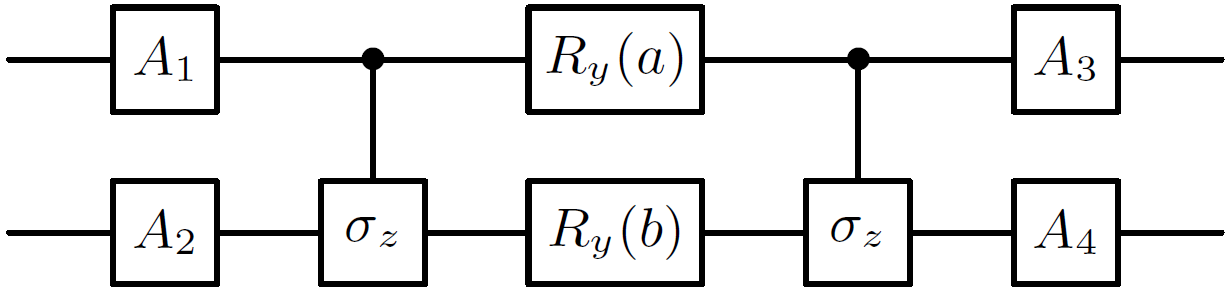
\includegraphics[width=\textwidth]{figure/two-qubit.png}
  \caption{Optimal Quantum Circuits for General Two-Qubit Gates are 15 single qubit gates and 3 CNOT gates\cite{two}}
\end{figure}
\end{frame}

\subsection{Introduction to Three-Qubit Quantum Gates}
\begin{frame}
\frametitle{Realization of Three-Qubit Quantum Gates}
\begin{itemize}
  \item universal gate family: $\{R_z,R_y,CNOT\}$
  \item basic idea: KAK Algorithm\cite{kak}, block-diagonal matrix
  \item results:98 single qubits and 40 CNOT gates
\end{itemize}
% introduce three qubit gates and the tools
\end{frame}

\subsection{Realization Techniques}
\subsubsection{Decomposition}
\begin{frame}
\frametitle{KAK Decomposition\cite{kak}}
any $SU(8)$ can be decomposed as
\begin{align}
  U&=K_{1} \exp \left(-i\left(\beta_{1} XXX+\beta_{2} YYX+\beta_{3} ZZX+\beta_{4} IIX\right)\right) K_{2}\\
  K_{1}&= P_{1}\exp \left(-i\left(\alpha_{1}XXX + \alpha_{2}YYZ + \alpha_{3}ZZZ\right)\right)P_{2},\\
  K_{1}&= P_{3}\exp \left(-i\left(\gamma_{1}XXX + \gamma_{2}YYZ + \gamma_{3}ZZZ\right)\right)P_{4}
\end{align}
% AKA results and step followed
\end{frame}
\begin{frame}
\frametitle{KAK Decomposition\cite{kak}}
\begin{figure}
  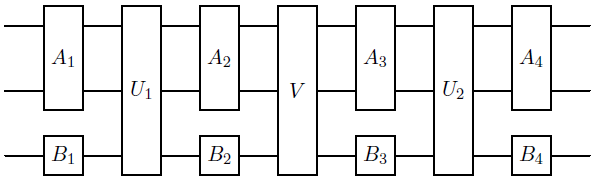
\includegraphics[width=.8\textwidth]{figure/three.png}
  \caption{KAK decomposition of a three-qubit unitary operation.}
\end{figure}
% AKA results and step followed
\end{frame}
\subsubsection{Diagonalization}
\begin{frame}
\frametitle{Diagonalization}
\begin{itemize}
  \item target:
  \begin{align}
    P=\begin{bmatrix}
      P_1 &&\\
      &P_1 &&\\
      &&P_2&\\
      &&&P_2
    \end{bmatrix}
  \end{align}
  % figure need of use matrix
  \item $\{CNOT,CZ,SWAP\}$
\end{itemize}
% how and results figure
\end{frame}

\begin{frame}
  \frametitle{Diagonalization}
  \begin{figure}
    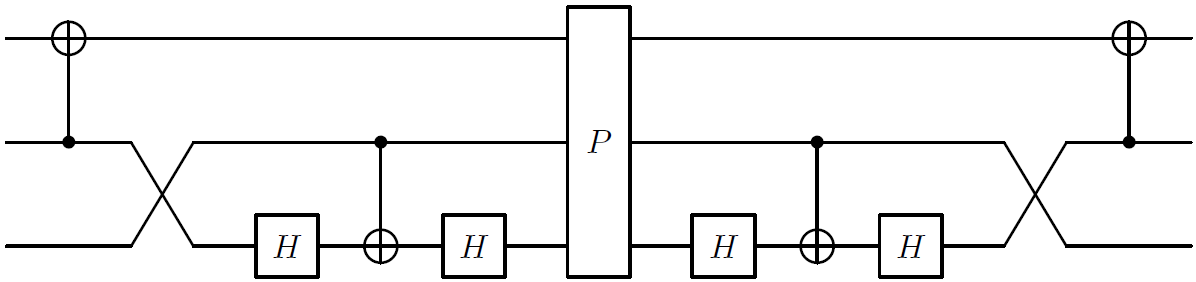
\includegraphics[width=.8\textwidth]{figure/N1.png}
    \caption{Decomposition of the unitary operation$\exp(i(a XXZ+b YYZ))$}
  \end{figure}

  \begin{figure}
    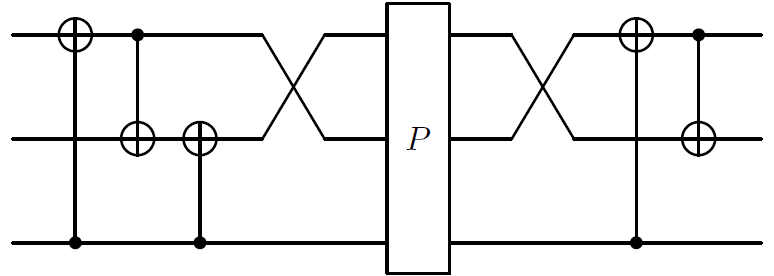
\includegraphics[width=.5\textwidth]{figure/M1.png}
    \caption{Decomposition of the unitary operation $\exp(i(\alpha_1 XXX+\alpha_2 YYX))$}
  \end{figure}
\end{frame}
\subsubsection{Block-Diagonalization}
\begin{frame}
\frametitle{Block-Diagonalization}
\begin{figure}
  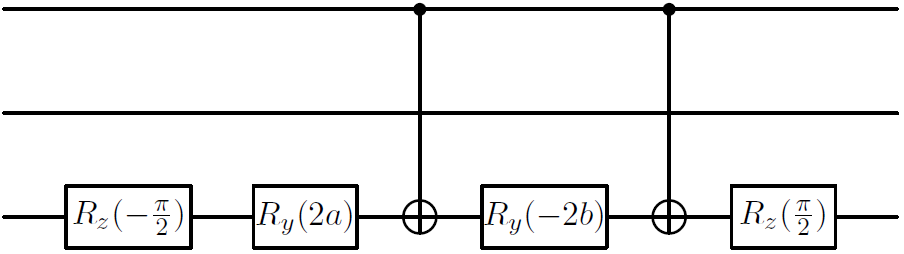
\includegraphics[width = .8\textwidth]{figure/P.png}
  \caption{a realization of Block-Diagonalization P}
\end{figure}
% result and way
\end{frame}
\begin{frame}
  \frametitle{whole circuit}
  \begin{figure}
    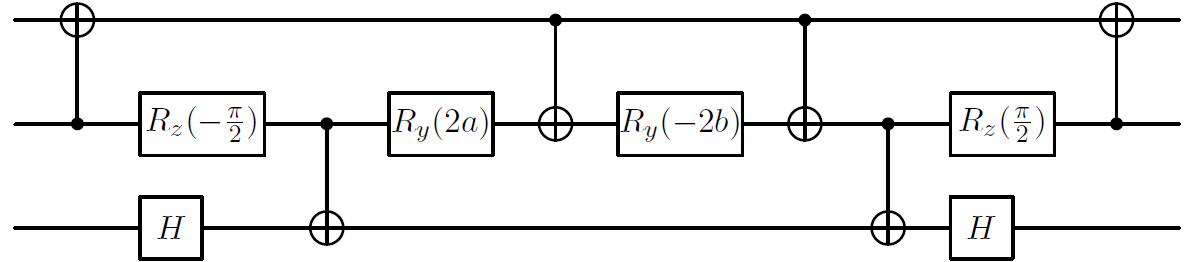
\includegraphics[width = .8\textwidth]{figure/N1wole.png}
    \caption{a realization of Block-Diagonalization P}
  \end{figure}
  \begin{figure}
    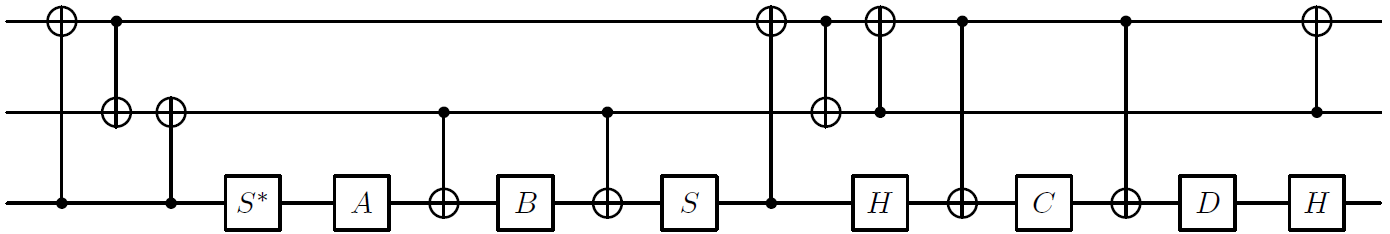
\includegraphics[width = .8\textwidth]{figure/M.png}
    \caption{a realization of Block-Diagonalization P}
  \end{figure}
\end{frame}
\subsubsection{Counter}
\begin{frame}
\frametitle{Counter}
  \begin{figure}
    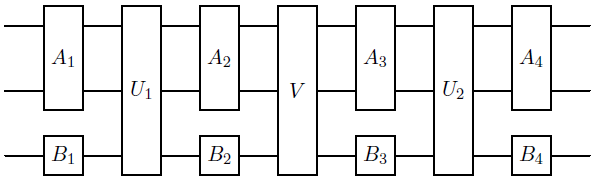
\includegraphics[width=.8\textwidth]{figure/three.png}
  \end{figure}

%  the whole number
\end{frame}

\section{QFAST Algorithm}

\subsection{Top-Down vs Bottom-Up Synthesizers}
\begin{frame}
\frametitle{Top-Down vs Bottom-Up Synthesizers}
\begin{figure}
  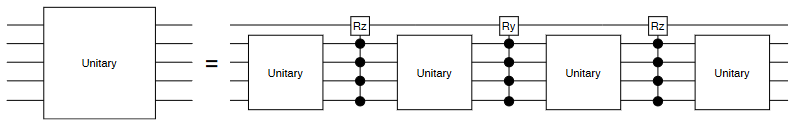
\includegraphics[width=\textwidth]{figure/top-down.png}
  \caption{Top-down synthesizers,decompose large unitaries into smaller ones while maintaining equality}
\end{figure}
% figure here
\end{frame}
\begin{frame}
  \frametitle{Top-Down vs Bottom-Up Synthesizers}
  \begin{figure}
    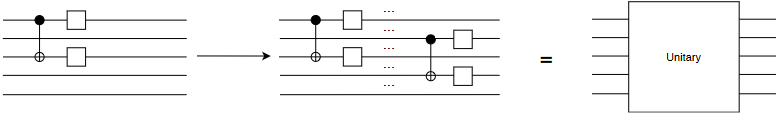
\includegraphics[width=\textwidth]{figure/bottom-up.png}
    \caption{Bottom-up synthesizers start with an empty circuit and build up to equality.}
  \end{figure}
  \begin{figure}
    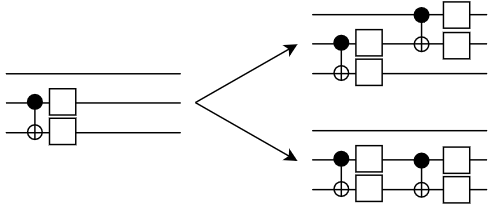
\includegraphics[width=.3\textwidth]{figure/Qsearch.png}
    \caption{QSearch uses native gates in synthesis and searches for structure in their circuit space.}
  \end{figure}
  % figure here
\end{frame}
\subsection{Introduction to QFAST Algorithm}
\begin{frame}
\frametitle{Basic idea to QFAST Algorithm}
\begin{itemize}
  \item use function to represent gates and circuits
  \item replaces expensive searches over circuit structures with numerical optimization
\end{itemize}
% work flow here
\end{frame}

\subsection{Gate Representation}
\begin{frame}
\frametitle{Gate Representation}

\begin{align}
  &F(Q, \vec{\alpha})=P_{Q}(G(\vec{\alpha}) \otimes I) P_{Q}^{T}\\
  &V(\vec{Q}, \vec{\alpha}, \vec{l})=\left(\sum_{Q \in \vec{Q}} l_{Q} \cdot P_{Q}\right)(G(\vec{\alpha}) \otimes I)\left(\sum_{Q \in \vec{Q}} l_{Q} \cdot P_{Q}^{T}\right)
\end{align}
where
\begin{align}
  G(\vec{\alpha})=e^{\mathrm{i}\left(\vec{\alpha} \cdot \sigma^{\vec{\otimes} n}\right)}
\end{align}
%  result formula
\end{frame}

\subsection{Cost Function for Optimization}
\begin{frame}
\frametitle{Cost Function for Optimization}
derive form Frobenius norm
\begin{align}
  \Delta\left(U_{C}, U_{T}\right)=1-\frac{\left|\operatorname{Tr}\left(U_{T}^{\dagger} U_{C}\right)\right|}{d}
\end{align}
% function here and how to optimize
\end{frame}
\begin{frame}
  \frametitle{work flow}
  \begin{itemize}
    \item decomposition
    \item instantiation
    \item recombination
  \end{itemize}
\end{frame}
\subsection{Comparison with Other Algorithms}
\begin{frame}
\frametitle{Comparison with Other Algorithms}
\begin{itemize}
  \item Evaluation Metrics:
  \begin{itemize}
    \item total CNOT gate count
    \item total count of single qubit gates
    \item critical path length
    \item average gate parallelism
    \item scalability and execution time
  \end{itemize}
  \item Benchmark: Transverse Field Ising Models
  \item 3-7 qubits
\end{itemize}
% how to compare and the metrics
\end{frame}
\begin{frame}
\frametitle{Comparison results}
compare with Qiskit on average:
\begin{itemize}
  \item $10\times$ fewer CNOT gates
  \item $5.2\times$ fewer U3 gates
  \item $5.7\times$ decrease of the circuit critical
  \item $1.03\times$ better parallelism
  \item $15\times$ slower than IBM Qiskit
\end{itemize}
\end{frame}
\begin{frame}
  \frametitle{Comparison results}

  \begin{table}[]
    \begin{tabular}{l|lll}
    tfim-7-20  & Qiskit mapped & Qiskit synthesized & QFAST  \\\hline
    singal gate    & 260           & 19360              & 89     \\
    CNOT           & 240           & 18653              & 41     \\
    critical patth & 152           & 89478              & 55     \\
    pararllelism   & 3.29          & 1.03               & 2.77   \\
    time           & 0.61          & 13222.11           & 307.57
    \end{tabular}
    \caption{In terms of ALL-to-ALL synthesis results. QFAST time out when running the tfim-7-40 and tfim-7-100 benchmark examples}
    \end{table}
\end{frame}
\begin{frame}
  \frametitle{Comparison results}

  \begin{table}[]
    \begin{tabular}{l|lll}
    tfim-7-20  & Qiskit mapped & Qiskit synthesized & QFAST  \\\hline
    ssingal gate    & 1300          & 89483              & 87      \\
    CNOT           & 1200          & 58316              & 40      \\
    critical patth & 712           & 82915              & 49      \\
    pararllelism   & 3.51          & 1.78               & 2.59    \\
    time           & 6.09          & 705.01             & 8208.44
    \end{tabular}
    \caption{In terms of Linear synthesis results.}
    \end{table}
\end{frame}
\subsection{Limitations}
\begin{frame}
\frametitle{Limitations}
...
% limitation here
\end{frame}

\section{Conclusion}
\begin{frame}
\frametitle{Summary}
...
% summary something
\end{frame}

\section{References}
\begin{frame}[noframenumbering,allowframebreaks,t]
	\frametitle{references}
	\printbibliography
\end{frame}
\begin{frame}
  \centering
  \Huge{END\\Thank you}
\end{frame}

\end{document}
